% -*- root: 00-main.tex -*-
\section*{Results and discussion}
\label{sec:results}

\subsection*{Proof of concept}
\label{sec:results_phantom}

Applying the evaluation protocol introduced in \autoref{sec:experiments_evaluation} on
  the ``cortex'' phantom (\autoref{fig:phantom}), we successfully tested the method and
  fine tuned the algorithm for its use on real data.
In this characterization experiment, we generated random smooth displacement fields $U^{-1}_{true}$
  (step 4 in \autoref{sec:experiments_evaluation}) based on a B-Spline field with
  control points evenly located in a $6 \times 6 \times 6$ grid covering the region of the phantom.
Invertibility is ensured by controlling the maximum	displacement
  \citep{rueckert_diffeomorphic_2006}.
The software tool to generate these fields is included with the released package.
In this experiment we used $\hat{U}_{cc} = (U^{-1}_{true})^{-1}$, i.e. the ground-truth
  displacement field.
We performed the experiment in two different realizations of the phantom, one at full resolution
  and a second with half resolution to study the performance under strong partial volume effect
  conditions.
The distorted phantoms and visual results are presented in \autoref{fig:results_phantom}.
Quantitative evaluation of the \gls*{swindex} is reported in \autoref{tab:swi_phantom}.

\begin{table}
	\caption{Quantitative evaluation on phantoms: \acrlong*{swindex}}
	\label{tab:swi_phantom}
    \begin{tabular}{llll}
    Voxel size  & Interior surface & Exterior surface & Average \\
    $1.0mm$ & $0.718mm$            & $0.724mm$            & $0.721mm$   \\
    $2.0mm$ & $0.723mm$            & $0.726mm$            & $0.725mm$   \\
    \end{tabular}
\end{table}

{\color{red}
\paragraph*{Convergence evindence and settings}
 discuss choice of $\tau$, Courant-Friedrichs-Lewy (CFL) condition / Wolfe conditions, multi-resolutions on the bspline grid, image samples and surface sampling,  etc.
\paragraph*{Efficient field densification}
As long as the dense deformation field is iteratively interpolated
from the same set of control points that define the $L-1$ contours,
it is possible to pre-cache all the $\psi_k(\vec{v}_i)$ weights into a
sparse matrix for fast densification. As well, we achieve a
diffeomorphic transform by}

% In regular intervals, after certain number of iterations,
% the parameters $\Theta_l$ of the regions can be reestimated
% based on the shifted volumetric samples
% $\vec{x}' = \vec{x_0} + u(\vec{x})$.




\begin{figure*}
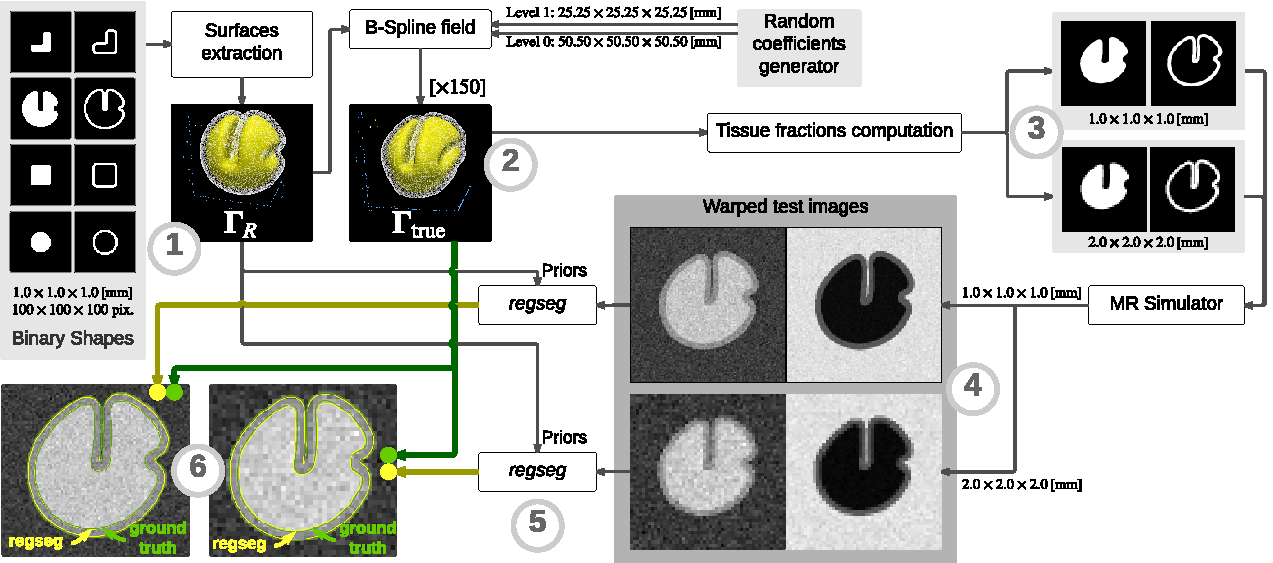
\includegraphics[width=\textwidth]{figures/figure03}
\caption{Proof of concept of the registration method. First row shows the registration experiment
  on the high-resolution ($1.0mm$ isometric) realization of the phantom, second row contains the
  low-resolution ($2.0mm$ isometric) version.
  Both phantoms were simulated with \gls*{snr} 30.
  In the first column, the distorted phantoms presented with the undistorted contours.
  For the second column, the contours have been replaced by the distorted contours using
    the ground-truth warping $U^{-1}_{true}$.
  The third column contains again the contours warped with the ground-truth field
  (thin yellow line), and the corresponding contours (green and blue thick lines)
  obtained with the presented method.
  Finally, last row represents the recovered images unwarped using the $\hat{U}_{tst}$
    found through our registration.
  }\label{fig:results_phantom}
\end{figure*}

\subsection*{Susceptibility distortion correction}
\label{sec:results_hcp}

As we propose the \gls*{fa} and the \gls*{md} as target features, we
  implemented a simplified pipeline for processing \gls*{dmri} using
  \emph{MRtrix} \citep{tournier_mrtrix_2012}.
\todo[inline]{insert here the summary of parameters}

Selecting the appropriate labels in the \emph{aparc} segmentation, we applied
  the marching-cubes algorithm again to extract priors of the following
  homogeneous regions in terms of \gls*{fa} and \gls*{md} joint distribution:
\begin{itemize}
	\item \gls*{csf} of the ventricular system,
	\item deep \gls*{gm} structures,
	\item \gls*{wm} surface as the ensemble of brain stem, and
	  cerebellar and cerebral \gls*{wm},
	\item cortical \gls*{gm} surface, including cerebellar \gls*{gm}.
\end{itemize}

\subsection*{Discussion}
\label{sec:discussion}
We propose a registration-segmentation algorithm designed for biomedical
  image analyses that are affected by all or some of the following circumstances:
  \begin{itemize}
  	\item Reference and target images do not present appropriate contrasts to
  	perform volume-based registration reliably, or there is not available an apt image
 		to be used as reference.
  	\item The low resolution of the target volume produces strong partial volume effects
  	that exclude the use of voxel-wise segmentation algorithms and hinder volume-based
  	registration.
  	\item The unknown warping is smooth enough to be represented with a sufficient number
  	of BSpline kernels, and its explicit need is justified (i.e. the distortion
  	field in \gls*{dmri} images, object tracking applications, etc.).
  \end{itemize}
The algorithm is designed for the proposed application on correcting distortions of
  \gls*{dmri} data, a required preliminary step to extract the structural connectivity
  networks.
As a consequence, our approach relies on the availability of precise segmentations or
  surfaces of the objects that are to be segmented on the target volume(s).
Connectome extraction protocols generally include the acquisition of \gls*{t1} images
  to provide with prior information about anatomy with high accuracy.
\todo[inline]{Add sentence about comment RW\#1 of IPMI2013: incorporate knowledge of
the EPI distortions into regularization}
Our method solves in a single step a joint problem usually addressed in two steps.
The first solves the linear registration of the \gls*{t1} and \gls*{dmri} data (i.e.
  \cite{greve_accurate_2009}), whereas the second corrects for the nonlinear distortions
  derived from the inhomogenety of magnetic susceptibility across tissues
  \citep{jezzard_correction_1995}.

{\color{red} We also considered the reproducibility of results a design requirement.
Therefore, real data are fetched from a publicly available repository
  (the Human Connectome Project \citep{essen_human_2012}) and all the software
  involved in this paper is also publicly released.
\autoref{fig:evworkflows} describes the general structure of the workflow we implemented
  as evaluation instrument, using \emph{nipype} \citep{gorgolewski_nipype_2011} to ensure
  reproducibility.}

We implemented the registration method upon the widely used Insight Registration and Segmentation
	Toolkit (\url{http://www.itk.org}) with the aim to release a useful and free software bundle.
The instrumentation framework is also distributed with the registration method,
  and has been implemented using \emph{nipype} \citep{gorgolewski_nipype_2011}.
The pipelines include the automatic generation of the ``cortex'' phantom.
The real datasets are publicly available under the \gls*{hcp} project.
Thus, all the experiments and results presented in this paper are intended to be
  fully reproducible.